\section{Schnyder Wälder}\label{sw}
Schnyder Wälder, im weiteren \textit{Schnyder Woods} wurden zuerst von Walter Schnyder zur Betrachung der Ordungs-Dimension planarer Graphen, als eine Färbung und Orientierung auf den inneren Kanten einer Triangulierung, betrachtet \cite{schnyder89}. In einem weiteren Resultat dienten sie zur Erlangung einer planaren Einbettung auf einem $n-2 \times n-2$ Netz\cite{schnyder90}. Im Folgenden werden wir die Verallgemeinerung auf drei-zusammenhängende plane Graphen durch Felsner \cite{felsner01} und die zu ihnen in Bijektion stehenden Schnyder Labelings einführen.\\
\begin{definition}[Schnyder Woods]
Ein Schnyder Wood ist eine Orientierung und Beschriftung der Kanten von $G$ mit den Labeln 1, 2 und 3 unter Berücksichtigung der folgenden Regeln\footnote{Alternativ kann hier auch anschaulicher einfach von rot, blau und grün gesprochen werden. Es wird davon ausgegangen, dass die Label zyklisch sortiert sind, sodass $i+1$ und $i-1$ immer definiert sind.}:
\begin{itemize}
\item[W1] Jede Kante ist entweder un- oder bigerichtet. Falls sie bigerichtet ist haben beide Richtungen unterschiedliche Label.
\item[W2] An jeder Aufhängung  $s_i$ exisitert eine nach ausssen gerichtete Kante ohne Endpunkt mit Label i.  
\item[W3] Jeder Knoten $v$ hat hat Ausgangsgrad eins zu jedem Label. Um $v$ existieren im Uhrzeigersinn eine Auskante mit Label 1, null oder mehr eingehende Kanten mit Label 3, eine Auskante mit Label 2, null oder mehr  eingehende Kanten mit Label 1, eine Auskante mit Label 2 und null oder mehr  eingehende Kanten mit Label 2.
\item[W4] Es existiert kein gerichteter Zykel mit einem Label.
\end{itemize}

\end{definition}

\begin{figure}[h]
	\centering
  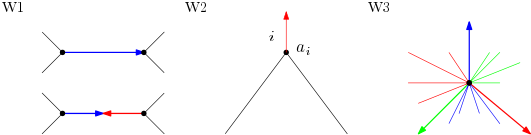
\includegraphics[width=0.98\textwidth]{schnyder_wood_def.png}
	\label{10_example}
\end{figure}

\begin{definition}[Schnyder Labeling]
Ein Schnyder Labeling ist eine Beschriftung Winkel von $G$ mit den Labeln 1, 2 und 3 unter Berücksichtigung der folgenden Regeln:
\begin{itemize}
\item[L1] Um jedes innere Gebiet bilden die Label im Uhrzeigersinn nichtleere Intervalle von 1en, 2en und 3en. Am äusseren Gebiet gilt dies gegen den Uhrzeigersinn.
\item[L2] Um jeden inneren Knoten bilden die Label im Uhrzeigersinn nichtleere Intervalle von 1en, 2en und 3en.
\item[L3] An Aufhängung $a_i$ haben äusseren Winkel die Label i-1 und i+1 im Uhrzeigersinn mit der halben Auskante dazwischen und die inneren Winkel das Label i.
\end{itemize} 

\end{definition}

\begin{theorem}
Schnyder Woods und Schnyder Labelings stehen in Bijektion zueinander.
// TODO  
\end{theorem}

// TODOBILD

\